%\documentclass[12pt,a4paper,oneside,openany]{memoir} 
% Skabelon af DTU's LaTeX support gruppe, v20090423

\usepackage[utf8]{inputenc} 
%\usepackage[danish]{babel} % danske overskrifter
\usepackage[T1]{fontenc}   % fonte (output)
\usepackage{lmodern}       % vektor fonte
\usepackage{fancybox, graphicx}      % indsættelse af billeder
\usepackage{palatino}      % lækker font
\usepackage{pdfpages}      % pdf som forside evt
\usepackage{todonotes}
\usepackage{microtype}
% \linespread{1.3}           % kræver lidt mere line spacing

\newcommand{\code}[1]{\texttt{#1}}
\newcommand{\HRule}{\rule{\linewidth}{0.5mm}}

%\addto\captionsdanish{
%  \renewcommand{\contentsname}%
%    {Indholdsfortegnelse}     %
%} % Så bruger vi bare 'Indholdsfortegnelse' i stedet for 'Indhold'


\usepackage{underscore}
\usepackage{pdflscape}
\usepackage{todonotes}

\usepackage[plainpages=false,pdfpagelabels,pageanchor=false]{hyperref} % aktive links
\def\sectionautorefname{afsnit}

\usepackage{memhfixc}  % rettelser til hyperref

\usepackage{tipa}
\pretolerance=2500     % højt tal, mindre orddeling og mere space mellem ord.
% 3000 er okey, 1000 er for lidt, 5000 i overkanten, 8000 er for meget..

\usepackage[font=small,labelfont=bf,labelsep=endash]{caption}
 
\pagestyle{headings}


\makechapterstyle{mortenovi}{%
\setlength{\beforechapskip}{0cm}%længde fra top af side til kapitel-overskrifter
\setlength{\afterchapskip}{1cm}%længde fra kapiteltekst til body-tekst
\setlength{\midchapskip}{2cm}%længe mellem kapitelnummer og kapiteltekst
\renewcommand\chapnamefont{\normalfont\Large\scshape\raggedleft}
\renewcommand\chaptitlefont{\normalfont\Huge\bfseries\sffamily}
\renewcommand\chapternamenum{}%default "kapitel"
\renewcommand\printchapternum{%
    \makebox[0pt][l]{%
    \hspace{0.4em}
    \resizebox{!}{4ex}{\chapnamefont\bfseries\sffamily\thechapter}}
    }%"kapitel. x"-linjen og dens boxe og bredder - prøv at sætte xyz ind først på de tre linjer respektivt.
\renewcommand\afterchapternum{\par\hspace{1.5cm}\hrule\vspace{0.5cm}}
\renewcommand\afterchaptertitle{\vskip\onelineskip \hrule\vskip\afterchapskip
}}
\chapterstyle{mortenovi}

\maxtocdepth{subsection} %Only parts, chapters and sections in the table of contents
\settocdepth{subsection}

% \includeonly{forord,testing} % Kompiler kun de kapitler du arbejder med.

\usepackage{listings}
\usepackage{color}

\renewcommand*\lstlistingname{Kode}

\definecolor{dkgreen}{rgb}{0,0.6,0}
\definecolor{gray}{rgb}{0.5,0.5,0.5}
\definecolor{mauve}{rgb}{0.58,0,0.82}

\lstset{frame=tb, %lr
  language=Java,
  aboveskip=3mm,
  belowskip=3mm,
  showstringspaces=false,
  columns=flexible,
  basicstyle={\small\ttfamily},
  numbers=none,
  numberstyle=\tiny\color{gray},
  keywordstyle=\color{blue},
  commentstyle=\color{dkgreen},
  stringstyle=\color{mauve},
  breaklines=true,
  breakatwhitespace=true,
  basicstyle=\tiny\ttfamily
}

\usepackage{cleveref}


\begin{document}
%\includepdf[fitpaper]{billeder/forside}


\begin{center}
\thispagestyle{empty}

% Upper part of the page. The '~' is needed because \\
% only works if a paragraph has started.

\textsc{\LARGE IT University of Copenhagen}\\[1.5cm]

\textsc{\Large BDSA 2014 }\\[0.5cm]

% Title
\HRule \\[0.4cm]
{ \huge \bfseries Assignment 36.1 \\ [0.1cm]
    %\large \\ [0.4cm] 
    }

\HRule \\[1.5cm]

% Author and supervisor
\begin{minipage}{1\textwidth}
\begin{center} \large
Anders Wind Steffensen - awis@itu.dk\\
Christopher Blundell - mail@itu.dk\\
Pierre Mandas - mail@itu.dk\\
\end{center}
\end{minipage}


\vfill

% Bottom of the page
{\large \today}

\end{center}

\frontmatter%

%\include{abastract}
%\include{preface}

%\tableofcontents* % stjernen betyder vi ikke har den med i vores indholdsfortegnelse
\newpage


\mainmatter%

%input chapters here

\section{Q2-4}
\emph{Draw a use case diagram for a ticket distributor for a train system. The system includes
two actors: a traveler who purchases different types of tickets, and a central computer
system that maintains a reference database for the tariff. Use cases should include
BuyOneWayTicket, BuyWeeklyCard, BuyMonthlyCard, and UpdateTariff. Also include
the following exceptional cases: TimeOut (i.e., traveler took too long to insert the right
amount), TransactionAborted (i.e., traveler selected the cancel button without
completing the transaction), DistributorOutOfChange, and DistributorOutOfPaper.

(Remember that a use case diagram consists of both the sticky man diagram as well as the use cases written in text using the template on p. 45 in [OOSE].)}


\HRule \\[0.4cm]
\textbf{Use case name:} BuyTicket
\HRule \\[0.4cm]
\textbf{Participating actors:}
\begin{list_type}
	\item Initiated by Traveler
	\item Communicates with CentralComputerSystem
\end{list_type}
\HRule \\[0.4cm]
\textbf{Flow of events:}
\begin{enumerate}
	\item Traveler initiates BuyOneWayTicket, BuyWeeklyCard or BuyMonthlyCard.
	\item Traveler pays for the ticket.
	\begin{enumerate}
		\item (Exceptional case) Timeout: Traveler took too long to insert the right amount of money. TicketDistributor has to abort.
		\item (Exceptional case) TransactionAborted: Traveler selected the cancel button without completing the transaction.
		\item (Exceptional case) DistributorOutOfChange: TicketDistributor is out of change, and can therefore not give back change to the Traveler, and has to abort.
		\item (Exceptional case) DistributorOutOfPaper: TicketDistributor is out of paper, and can therefore not print out the ticket for the Traveler, and has to abort.
	\end{enumerate}
	\item UpdateTariff is initiated, and the database is being updated.
\end{enumerate}
\HRule \\[0.4cm]
\textbf{Entry condition:} Traveler interacts with the TicketDistributor.
\HRule \\[0.4cm]
\textbf{Exit condition:}
\begin{enumerate}
	\item Traveler has received the ticket and change (if any).
	\item Traveler has initiated TransactionAborted.
	\item TicketDistributor has initiated DistributorOutOfChange OR DistributorOutOfPaper.
\end{enumerate}
\HRule \\[0.4cm]
\textbf{Quality Requirements:}
\HRule \\[0.4cm]

\section{Q2-4.1}
\emph{Draw the class diagram for the ticket distributor system from exercise 2-4.}
\\
\emph{Class Diagram}
\\
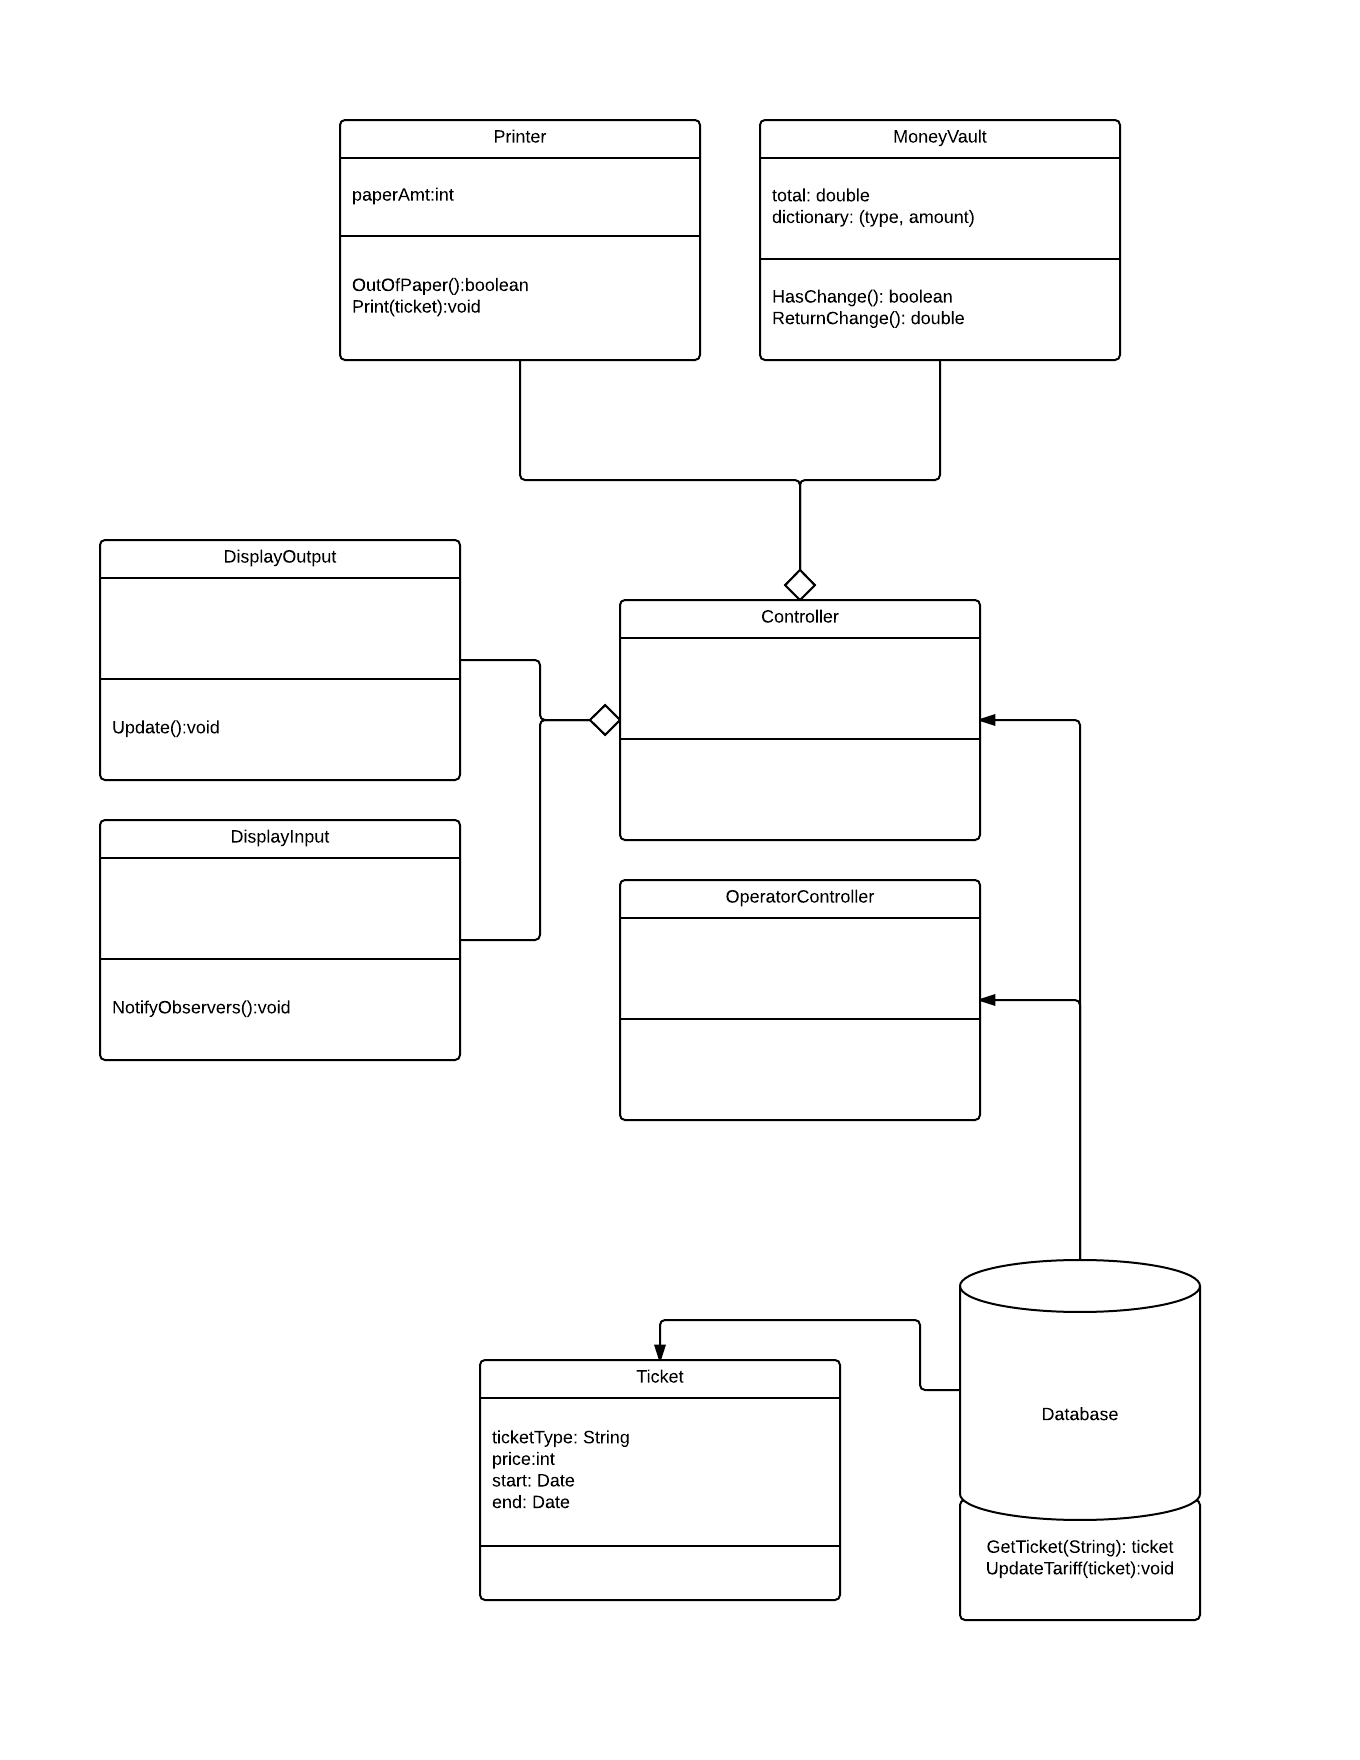
\includegraphics[scale=0.2]{Assignment-36-Class-Diagram}
\section{Q2-4.2}
\emph{Draw the sequence diagram for the use case in exercise 2-4.}
\section{Q2-4.3}
\emph{Draw an activity diagram showing how a traveler buys a ticket.}


\end{document}